\item {\bf Linear regression: linear in what?}

In the first two lectures, you have seen how to fit a linear function of the data for the regression problem.  In this question, we will see how linear regression can be used to fit non-linear functions of the data using feature maps. We will also explore some of its limitations, for which future lectures will discuss fixes.

\begin{enumerate}
	\item \points{2a} {\bf Learning degree-3 polynomials of the input}

Suppose we have a dataset $\{(x^{(i)}, y^{(i)})\}_{i=1}^{\nexp}$ where $x^{(i)}, y^{(i)} \in \mathbb{R}$. We would like to fit a third degree polynomial $h_{\theta}(x) = \theta_3x^3 + \theta_2x^2 + \theta_1x^1 + \theta_0$ to the dataset. The key observation here is that the function $h_{\theta}(x)$ is still linear in the unknown parameter $\theta$, even though it's not linear in the input $x$. This allows us to convert the problem into a linear regression problem as follows. 
	
Let $\phi:\mathbb{R}\rightarrow \mathbb{R}^4$ be a function that transforms the original input $x$ to a $4$-dimensional vector defined as
\begin{align}
\phi(x) = \left[\begin{array}{c} 1\\ x \\ x^2 \\ x^3 \end{array}\right]\in \mathbb{R}^4 \label{eqn:feature}
\end{align}
Let $\hat{x}\in \mathbb{R}^4$ be a shorthand for $\phi(x)$, and let $\hat{x}^{(i)} \triangleq \phi(x^{(i)})$ be the transformed input in the training dataset. We construct a new dataset $\{(\phi(x^{(i)}), y^{(i)})\}_{i=1}^{\nexp} = \{(\hat{x}^{(i)}, y^{(i)})\}_{i=1}^{\nexp}$ by replacing the original inputs $x^{(i)}$'s by $\hat{x}^{(i)}$'s.  We see that fitting $h_{\theta}(x) = \theta_3x^3 + \theta_2x^2 + \theta_1x^1 + \theta_0$ to the old dataset is equivalent to fitting a linear function $h_{\theta}(\hat{x}) = \theta_3\hat{x}_3 +  \theta_2\hat{x}_2 + \theta_1\hat{x}_1 + \theta_0$ to the new dataset because 
\begin{align}
h_\theta(x) =  \theta_3x^3 + \theta_2x^2 + \theta_1x^1 + \theta_0 =  \theta_3 \phi(x)_3 + \theta_2\phi(x)_2 + \theta_1\phi(x)_1 + \theta_0 = \theta^T \hat{x}
\end{align}
	
In other words, we can use linear regression on the new dataset to find parameters $\theta_0,\dots, \theta_3$.

Please write down 1) the objective function $J(\theta)$ of the linear regression problem on the new dataset $\{(\hat{x}^{(i)}, y^{(i)})\}_{i=1}^{\nexp}$ and 2) the update rule of the batch gradient descent algorithm for linear regression on the dataset $\{(\hat{x}^{(i)}, y^{(i)})\}_{i=1}^{\nexp}$. 

\textit{Terminology:} 	In machine learning, $\phi$ is often called the feature map which maps the original input $x$ to a new set of variables. To distinguish between these two sets of variables, we will call $x$ the input {\bf attributes}, and call $\phi(x)$ the {\bf features}. (Unfortunately, different authors use different terms to describe these two things. In this course, we will do our best to follow the above convention consistently.)

	\item \points{2b} {\bf Degree-k polynomial regression}


For this sub-question question, we will use the datasets provided in
the following file:
%
\begin{center}
	\texttt{src/train.csv}
\end{center}
%

This file contains two columns: $x$ and $y$. In the terminology described in the introduction, $x$ is the attribute (in this case one dimensional) and $y$ is the output label.

Using the formulation of the previous sub-question, implement linear regression with \textbf{normal equations} using the feature map of degree-k polynomials. Using the |LinearModel| provided in |src/submission.py|, this means you will be implementing the functions |fit()|, |predict()|, and |create_poly()|.  

To extend the idea above to degree-$k$ polynomials, consider $\phi:\mathbb{R}\rightarrow \mathbb{R}^{k+1}$ to be 
		\begin{align}
	\phi(x) = \left[\begin{array}{c} 1\\ x \\ x^2\\ \vdots \\x^k \end{array}\right]\in \mathbb{R}^{k+1} \label{eqn:feature-k}
	\end{align}

We will use $k=1,2,3,5,10,20$ as test cases. To verify a correct implementation, autograder test case |2b-9-basic| will create a plot in |src/large-poly.png|.  Note that test |2b-9-basic| will NOT be awarded points and is used to test if your implementation can generate a plot similar to the following:

\begin{figure}[H]
  \centering
  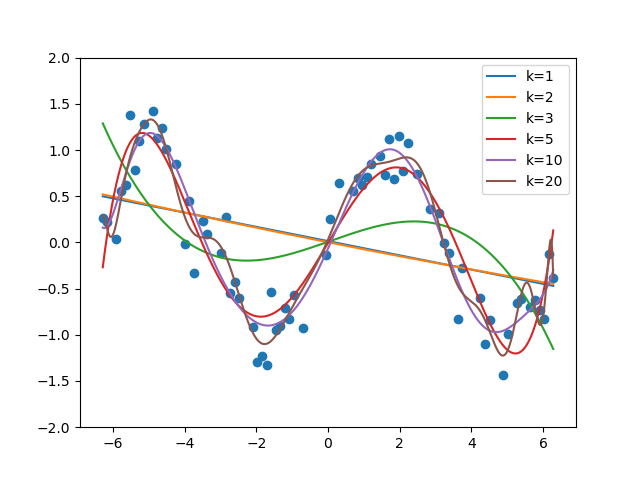
\includegraphics[width=0.65\linewidth]{02-featuremaps/large-poly.png}
  \centering
\caption{Polynomial regression with kernel sizes 1,2,3,5,10 and 20}
\end{figure}

  \item \points{2c}

Regarding question 2.b, briefly comment on your observations of the fit for each K value.

  \item \points{2d} {\bf Other feature maps}

You may have observed that it requires a relatively high degree $k$ to fit the given training data, and this is because the dataset cannot be explained (i.e., approximated) very well by low-degree polynomials. By visualizing the data, you may have realized that $y$ can be approximated well by a sine wave. In fact, we generated the data by sampling from $y = \sin(x) + \xi$, where $\xi$ is noise with Gaussian distribution. Please update the feature map $\phi$ to include a sine transformation as follows:

\begin{align}
\phi(x) = \left[\begin{array}{c} \sin(x) \\ 1 \\ x \\ x^2\\ \vdots \\x^k\end{array}\right]\in \mathbb{R}^{k+2} \label{eqn:feature-sine}
\end{align}

Complete the function |create_sin()| in |src/submission.py| to implement the updated feature map.  Again, ensure your code  works with a general $k$.  We will use $k=1,2,3,5,10,20$ as test cases. To verify a correct implementation, autograder test case |2d-7-basic| will create a plot in |src/large-sine.png|. Note that test |2d-7-basic| will NOT be awarded points and is used to test if your implementation can generate a plot similar to the following:

\begin{figure}[H]
  \centering
  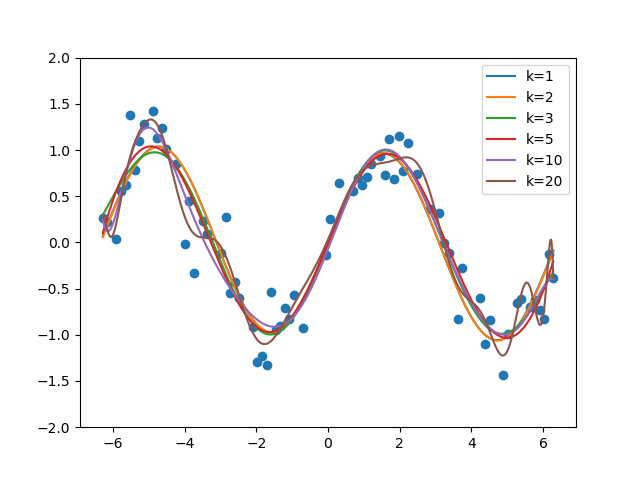
\includegraphics[width=0.65\linewidth]{02-featuremaps/large-sine.png}
  \centering
\caption{Polynomial regression with other features with kernel sizes 1,2,3,5,10 and 20}
\end{figure}


  \item \points{2e}

Compare the fitted models for 2.d with those from 2.b, and briefly comment about noticeable differences in the fit with this feature map.

  \item \points{2f} {\bf Overfitting with expressive models and small data}

You will not be required to code, write, or submit anything for this sub-question.  For this and the remaining sub-questions, we will consider a small
dataset (a random subset of the dataset you have been using so far) with much fewer examples, provided in
the following file:
%
\begin{center}
	\texttt{src/small.csv}
\end{center}
%

We will be exploring what happens when the number of features start becoming bigger than the number of 
examples in the training set. Run your algorithm on this small dataset using the following feature map 
\begin{align}
\phi(x) = \left[\begin{array}{c} 1\\ x \\ x^2\\ \vdots \\x^k \end{array}\right]\in \mathbb{R}^{k+1} 
\end{align}
with $k = 1,2,3,5,10,20$ using the autograder test case |2f-0-basic|, which will create plots in |src/smalle-poly.png| and |src/small-sine.png|. 

\textbf{Remark: } The phenomenon you observe where the models start to fit the training dataset very well, but suddenly ``goes wild'' is due to what is called \emph{overfitting}. The intuition to have for now is that, when the amount of data you have is small relative to the expressive capacity of the family of possible models (that is, the hypothesis class, which, in this case, is the family of all degree $k$ polynomials), it results in overfitting.  

Loosely speaking, the set of hypothesis function is ``very flexible'' and can be easily forced to pass through all your data points especially in unnatural ways. In other words, the  model explains the noises in the training dataset, which shouldn't be explained in the first place. This hurts the predictive power of the model on test examples. We will describe overfitting in more detail in future lectures when we cover learning theory and bias-variance tradeoffs.\\

Your plots should look similar to the following:
\begin{figure}[H]
  \centering
  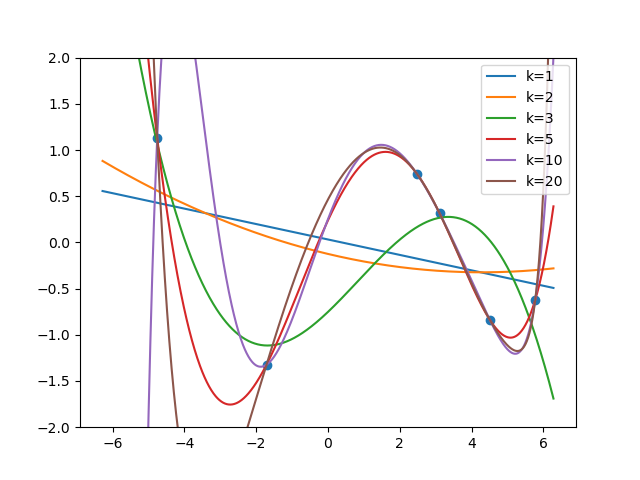
\includegraphics[width=0.65\linewidth]{02-featuremaps/small-poly.png}
  \caption{Polynomial regression with kernel sizes 1,2,3,5,10 and 20
  on small dataset}
  
  \centering
  \vspace{2mm}
  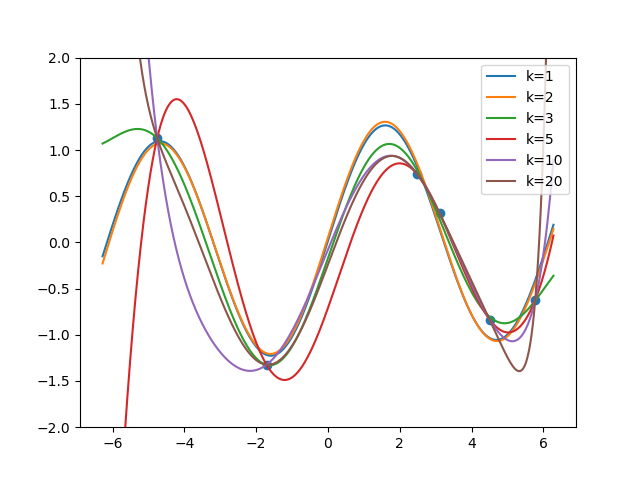
\includegraphics[width=0.65\linewidth]{02-featuremaps/small-sine.png}
  \centering
  \caption{Regression with other polynomial and sinusoidal features with kernel sizes 1,2,3,5,10 and 20
  on small dataset}
\end{figure}


  \item \points{2g}

Regarding question 2.f, observe and comment on how the fitting of the training dataset changes as $k$ increases.
\end{enumerate}
